% Faithful conversion from FullPaper_ RBL AI cclassification.docx.
% The supplied Springer LLNCS document class and running-head option are preserved.
\documentclass[runningheads]{llncs}

\usepackage{graphicx}
% Required by the source equations (\text, aligned math, and blackboard-bold symbols).
\usepackage{amsmath}
\usepackage{amssymb}
\usepackage{booktabs}
\usepackage{tabularx}
\usepackage{array}
\newcolumntype{Y}{>{\raggedright\arraybackslash}X}
\newcolumntype{C}{>{\centering\arraybackslash}X}
\emergencystretch=3em

\begin{document}

\title{AI-Based Classification of Functional and Non-Functional Requirements Using Selective ELECTRA--RoBERTa Fusion}
\titlerunning{Selective ELECTRA--RoBERTa Fusion for Requirements Classification}
\author{Quach The Duong}
\authorrunning{Q. T. Duong}
\institute{FPT University, Viet Nam}
\maketitle

\begin{abstract}
Automated classification of software requirements is complicated by short requirement statements, overlapping quality attributes, and severe class imbalance. This study proposes Selective ELECTRA--RoBERTa Fusion (SERF), a two-stage transformer architecture for multiclass classification of functional and non-functional requirements. SERF first applies an ELECTRA-based selector and uses its prediction directly when confidence and margin are sufficiently high and the predicted class is not in the predefined risky-class set. Other predictions are instead processed by an independently trained ELECTRA--RoBERTa fusion branch. The model was evaluated in the 969-instance PROMISE\_EXP dataset with 12 requirement categories. Under the three-seed no-augmentation protocol, SERF achieved an accuracy of \(0.8653 \pm 0.0105\), a weighted F1 of \(0.8595 \pm 0.0117\), and a Macro-F1 of \(0.7770 \pm 0.0307\). Its mean Macro-F1 exceeded those of RoBERTa and static ELECTRA--RoBERTa fusion by 4.91 and 2.16 percentage points, respectively. SERF routed \(36.76\%\) of test instances to fusion, corresponding to an architecture-derived estimate of 1.735 encoder invocations per requirement and a 13.24\% reduction relative to always-on static fusion. Training-set augmentation reduced mean Macro-F1 by 7.75 percentage points, indicating that its effect was model-dependent. These findings position selective fusion as a class-balanced performance and average active-encoder computation trade-off.
\keywords{software requirements classification \and non-functional requirements \and transformer models \and selective fusion \and ELECTRA \and RoBERTa \and class imbalance.}
\end{abstract}

\section{Introduction}\label{sec:introduction}

Requirements engineering establishes the functions, constraints, and quality attributes that guide software design, implementation, testing, and maintenance. Functional requirements describe the services or behaviors provided by a system, whereas non-functional requirements capture quality attributes and operational constraints such as security, usability, performance, availability, and maintainability. Accurate classification facilitates traceability and architecture-oriented analysis, but manual classification remains time-consuming and susceptible to inconsistent interpretation because requirements are predominantly expressed in natural language \cite{kaur_ai_requirements,shreda_nfr_nlp,kassab_ensemble_requirements}.

Early automated approaches relied on statistical representations, including bag-of-words and TF-IDF, together with classifiers such as Support Vector Machines, Logistic Regression, Decision Trees, and Random Forests \cite{shreda_nfr_nlp,idate_ml_requirements}. Although these methods provide useful and comparatively inexpensive baselines, they depend strongly on lexical features and may fail to represent contextual relationships in short or ambiguous statements. Pretrained transformer models address part of this limitation through contextual language representations. BERT, RoBERTa, ELECTRA, XLNet, and their variants have consequently been investigated for binary FR/NFR identification and fine-grained NFR classification \cite{kaur_ai_requirements,khan_transfer_requirements,shafikuzzaman_fewshot_requirements}.

Requirements classification remains constrained by severe class imbalance and ambiguity in short, semantically similar statements, while the effects of lexical augmentation may vary across model architectures \cite{lima_promise_exp,said_functional_nonfunctional,wei_eda}. Static hybrid models can combine complementary representations, but they activate every encoder for every input and consequently increase inference demand \cite{said_functional_nonfunctional}. Accordingly, this study proposes Selective ELECTRA--RoBERTa Fusion (SERF), a validation-controlled model that conditionally uses an ELECTRA-only prediction or an independent ELECTRA--RoBERTa fusion prediction.

The study addresses the following research questions:

\textbf{RQ1:} How effectively can pretrained transformer models classify software requirements across functional and multiple non-functional categories under class imbalance?

\textbf{RQ2:} How does the proposed SERF model compare with single-encoder and static hybrid transformer baselines in terms of class-balanced performance and seed-level stability?

\textbf{RQ3:} How do confidence- and class-aware selective routing and training-set augmentation affect classification performance and active inference demand?

The main contributions are as follows. First, the study presents a comparative evaluation of single-transformer, static hybrid, and selectively routed models on PROMISE\_EXP. Second, it introduces and evaluates SERF under a validation-controlled protocol. Third, it evaluates the proposed model using Macro-F1, per-class behavior, seed-level stability, augmentation ablation, route-to-fusion rate, and an architecture-derived encoder-invocation proxy. Finally, it reports the limitations of the experimental evidence explicitly and does not infer statistical or hardware-level superiority from descriptive comparisons.

The remainder of the paper reviews relevant classification approaches, describes the proposed methodology and experimental protocol, reports the empirical results, discusses their implications and limitations, and concludes with answers to the research questions and directions for further investigation.

\section{Related Work}\label{sec:related-work}
 

Conventional requirements classification commonly combines statistical text representations with supervised classifiers. Shreda and Hanani evaluated TF-based, TF-IDF, Word2Vec, and BERT-derived features on unconstrained requirement documents. Statistical representations produced accuracies between 84\% and 87\%, whereas semantic embeddings achieved between 88\% and 92\%; fusion of feature-specific models further improved the best individual result by 2.4\% \cite{shreda_nfr_nlp}. Idate et al. compared Logistic Regression, SVM, Decision Trees, Random Forests, and multilayer perceptrons and additionally applied cosine similarity to reject text unrelated to software requirements \cite{idate_ml_requirements}.

A systematic mapping by Kaur and Kaur identified SVM and CNN as frequently adopted classifiers and reported increasing use of transfer-learning methods \cite{kaur_ai_requirements}. However, the review also found limited evidence concerning deployment in complex, real-world environments. Conventional models therefore remain valuable as transparent and computationally economical baselines, but their dependence on surface-level representations restricts their ability to capture contextual differences between semantically related requirement categories.
 

BERT introduced deep bidirectional contextual pretraining, while RoBERTa revised the BERT training procedure through additional data and modified pretraining choices \cite{devlin_bert,liu_roberta}. ELECTRA instead learns through replaced-token detection, providing a discriminative pretraining objective distinct from masked-language modeling \cite{clark_electra}. These differences motivate comparative and hybrid investigation in requirements classification.

Khan et al. evaluated XLNet, BERT, DistilBERT, DistilRoBERTa, ELECTRA-base, and ELECTRA-small for NFR classification and reported their strongest result with XLNet \cite{khan_transfer_requirements}. Shafikuzzaman et al. subsequently compared zero-shot, few-shot, and generative language models across PROMISE and SecReq tasks. Their findings showed that few-shot models generally performed more consistently than zero-shot alternatives, while qualitative analysis identified insufficient context and annotation problems as recurrent error sources \cite{shafikuzzaman_fewshot_requirements}. These studies demonstrate the value of contextual representations but also show that performance depends on the classification setting, label distribution, and availability of task-specific examples.
 

Hybrid models seek to combine representations or decisions produced by different learners. Shreda and Hanani demonstrated that fusing classifiers trained on heterogeneous textual features could improve performance over individual models \cite{shreda_nfr_nlp}. Said et al. proposed feature-level fusion between BERT and RoBERTa and evaluated it on PROMISE and PROMISE\_EXP, reporting improvements in macro-averaged performance for their experimental protocol \cite{said_functional_nonfunctional}. At the LLM level, Kassab and Belbach combined four models through weighted voting and stacking, illustrating a decision-level alternative to representation fusion \cite{kassab_ensemble_requirements}.

Data augmentation has also been used to address limited and imbalanced training data. EDA introduced synonym replacement, random insertion, random swapping, and random deletion for text classification \cite{wei_eda}. Said et al. adapted related transformations to requirement statements and applied augmentation only to the training partition \cite{said_functional_nonfunctional}. However, improvements observed for one architecture or dataset do not establish that lexical augmentation is universally beneficial, particularly when short requirements contain modal verbs, numerical constraints, and domain-specific terms that may be altered by synthetic transformations.

Dynamic inference methods reduce computation by allocating different processing depths to different inputs. DeeBERT, for example, enables confident instances to exit from intermediate Transformer layers instead of traversing the complete network \cite{xin_deebert}. However, conditional representation fusion has received limited attention in requirements classification.

Within the examined requirements-classification literature, static fusion, ensemble prediction, and pretrained language models have been studied primarily from a predictive-performance perspective \cite{khan_transfer_requirements,shafikuzzaman_fewshot_requirements,kassab_ensemble_requirements,said_functional_nonfunctional}. Their evaluations do not jointly examine class-aware selective fusion, route-to-fusion behavior, augmentation sensitivity, and multi-seed class-balanced performance. This leaves an empirical gap concerning whether selective fusion can balance predictive performance, stability, and active inference demand under class imbalance.

\section{Methodology}\label{sec:methodology}

The overall research methodology is illustrated in Fig.~\ref{fig:serf-framework}. The workflow comprises minimal text normalization, stratified data splitting, controlled training and comparison of baseline, static hybrid, and SERF configurations, and evaluation of classification performance, route-to-fusion behavior, seed-level stability, and average active inference complexity.

\begin{figure}[t]
\centering
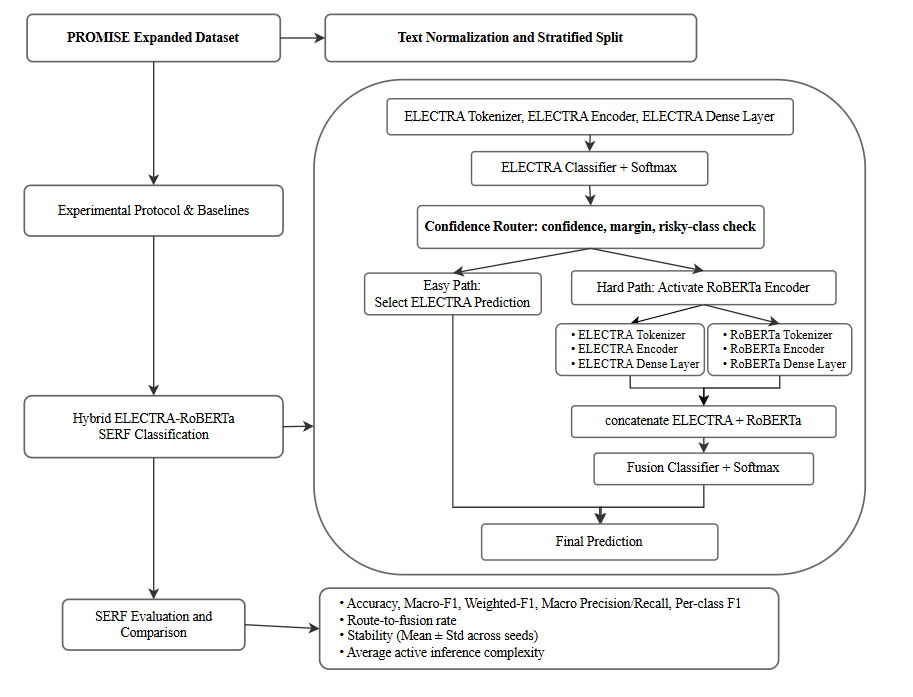
\includegraphics[width=0.95\textwidth]{figures/serf_framework.png}
\caption{Overview of the Proposed Selective ELECTRA--RoBERTa Classification Framework and the research pipeline.}
\label{fig:serf-framework}
\end{figure}

\subsection{Dataset Preprocessing}\label{sec:dataset-preprocessing}

PROMISE\_EXP \cite{lima_promise_exp} is used as the multiclass benchmark, with its class distribution reported in Table~\ref{tab:class-distribution}. Only minimal normalization is applied to preserve modal expressions, numerical constraints, and domain-specific tokens; the exact preprocessing operations are documented in Appendix~\ref{app:training-configurations}.

Preprocessing and augmentation follow the leakage-controlled partitioning protocol described in Sect.~\ref{sec:dataset-splitting}. When augmentation is used, it is confined to the training partition \cite{said_functional_nonfunctional,wei_eda}.

\begin{table}[!t]
\caption{Class Distribution of the PROMISE\_EXP Dataset}\label{tab:class-distribution}
\centering
\setlength{\tabcolsep}{4pt}
\small
\begin{tabular}{lcrr}
\toprule
\textbf{Full Name} & \textbf{Abbreviation} & \textbf{Count} & \textbf{Percentage  (\%)} \\
\midrule
Functional & F & 444 & 45.82 \\
Security & SE & 125 & 12.90 \\
Usability & US & 85 & 8.77 \\
Operational & O & 77 & 7.95 \\
Performance & PE & 67 & 6.91 \\
Look and Feel & LF & 49 & 05.06 \\
Availability & A & 31 & 3.20 \\
Maintainability & MN & 24 & 2.48 \\
Scalability & SC & 22 & 2.27 \\
Fault Tolerance & FT & 18 & 1.86 \\
Legal & L & 15 & 1.55 \\
Portability & PO & 12 & 1.24 \\
\bottomrule
\end{tabular}
\end{table}

\newpage
\subsection{Imbalance Handling Strategy}\label{sec:imbalance-handling}

The imbalance shown in Table~\ref{tab:class-distribution} is addressed through training-set augmentation and class-weighted learning. Transformer models incorporate weights computed from the training distribution into the cross-entropy loss. Augmentation is treated as an experimental factor rather than an assumed improvement; its transformations and class-support targets are documented in Appendix~\ref{app:training-configurations}.

\subsection{Baseline and Static Hybrid Models}\label{sec:baselines}

The comparison includes the single-transformer BERT, RoBERTa, ELECTRA, and ModernBERT models \cite{devlin_bert,liu_roberta,clark_electra}, together with static hybrid configurations. These baselines represent individual contextual encoders and always-on fusion strategies.

The proposed hybrid architecture is based on ELECTRA and RoBERTa because their representations are expected to be complementary. RoBERTa provides robust contextual semantic representations, whereas ELECTRA captures discriminative token-level signals that may help distinguish short and semantically similar requirement statements. For fair comparison, all transformer-based models use the first-token representation from the last hidden layer rather than pooler outputs. 

A static ELECTRA--RoBERTa model independently encodes each requirement and classifies the concatenated first-token representations \cite{said_functional_nonfunctional}. The complete fusion-head structure is reported in Appendix~\ref{app:training-configurations}.

\subsection{Proposed SERF Architecture}\label{sec:serf-architecture}

Selective ELECTRA--RoBERTa Fusion (SERF) comprises two independently trained components: an ELECTRA-only selector and an ELECTRA--RoBERTa fusion branch. The selector produces class logits from the first-token ELECTRA representation. Its prediction is retained when the confidence and margin satisfy the routing thresholds and the predicted label is not in the predefined risky-class set. Otherwise, the hard branch independently recomputes ELECTRA and RoBERTa representations, concatenates them, and produces replacement logits through the fusion classifier. The selector representation is not reused by the hard branch. In the implemented data pipeline, both tokenized views are prepared before routing; selectivity applies to encoder execution rather than tokenization. This mechanism avoids executing the fusion-branch encoders for easy-path instances while reserving the independently trained dual-encoder branch for uncertain or predefined risky-class predictions.

\section{Experimental Evaluation}\label{sec:experimental-evaluation}

\subsection{Experimental Setup}\label{sec:experimental-setup}

The experiments were implemented using PyTorch and Hugging Face Transformers. Scikit-learn was used for stratified dataset splitting, class-weight calculation, and evaluation, while Pandas and NumPy supported data processing and multi-seed result aggregation. Additional implementation details and software reproducibility notes are provided in Appendix~\ref{app:software-reproducibility}.

Balanced class weights were calculated exclusively from the training data available to each experimental variant. In the frozen variants, the lower eight Transformer layers were frozen to reduce computational cost and mitigate overfitting on short requirements. Complete configurations are reported in Appendix~\ref{app:training-configurations}.

The SERF selector and fusion branch were trained separately. Routing thresholds were selected exclusively on the validation set by maximizing Macro-F1, with route-to-fusion rate and accuracy used for tie-breaking. The threshold grid and risky-class set are reported in Appendix~\ref{app:training-configurations}.

\subsection{Dataset Splitting and Evaluation Protocol}\label{sec:dataset-splitting}

The 969 requirements across 12 classes were divided by stratified sampling with a fixed split seed of 42 \cite{lima_promise_exp}:

\[
70\%~\text{training} \;(678),\quad
15\%~\text{validation} \;(145),\quad
15\%~\text{testing} \;(146).
\]

The fixed partition preserved class proportions across training seeds, isolating variation due to initialization and training order. Splitting preceded augmentation, which was restricted to the training set; validation and test data remained unchanged, and class weights were computed from the resulting training frame.

RoBERTa, static ELECTRA--RoBERTa, and SERF used seeds 42, 123, and 2024, whereas other baselines primarily retained seed 42. Multi-seed comparisons are therefore restricted to configurations with all three runs. The held-out test set was accessed only after checkpoint and SERF-threshold selection on validation data. Macro-F1 was the primary metric under class imbalance, complemented by accuracy, weighted and macro-averaged measures, per-class F1, confusion matrices, mean \(\pm\) standard deviation, and the SERF route-to-fusion rate. Formal definitions are provided in Appendix~\ref{app:evaluation-definitions}.

\subsection{Main Performance Results}\label{sec:main-results}

Table~\ref{tab:serf-main-performance} reports the three-seed test performance of the unaugmented SERF configuration, which serves as the reference condition. Data augmentation is examined separately in Sect.~\ref{sec:augmentation-ablation}.

\begin{table}[!t]
\caption{Main test performance of SERF without augmentation across three seeds.}\label{tab:serf-main-performance}
\centering
\setlength{\tabcolsep}{4pt}
\small
\begin{tabular}{lc}
\toprule
\textbf{Performance metric} & \textbf{Mean \ensuremath{\pm} standard deviation} \\
\midrule
Accuracy & 0.8653 \ensuremath{\pm} 0.0105 \\
Weighted Precision & 0.8767 \ensuremath{\pm} 0.0127 \\
Weighted Recall & 0.8653 \ensuremath{\pm} 0.0105 \\
Weighted-F1 & 0.8595 \ensuremath{\pm} 0.0117 \\
Macro Precision & 0.8362 \ensuremath{\pm} 0.0340 \\
Macro Recall & 0.7695 \ensuremath{\pm} 0.0366 \\
\textbf{Macro-F1} & \textbf{0.7770 \ensuremath{\pm} 0.0307} \\
\bottomrule
\end{tabular}
\end{table}

The gap between weighted and macro-averaged metrics indicates that aggregate performance was influenced by the majority class. Macro Recall was also lower than Macro Precision, suggesting conservative predictions for underrepresented categories.

Accuracy remained comparatively stable across seeds, whereas Macro-F1 varied more strongly. This pattern suggests that initialization primarily affected minority-class predictions and supports reporting multi-seed summary statistics rather than a single run.

\subsection{Augmentation Ablation Results}\label{sec:augmentation-ablation}

An augmentation ablation was conducted to determine whether synthetic training instances improved SERF performance. Both conditions followed the protocol in Sect.~\ref{sec:dataset-splitting} and differed only in the use of training-set augmentation.

\begin{table}[!hb]
\caption{Three-seed augmentation ablation for SERF.}\label{tab:serf-augmentation-ablation}
\centering
\setlength{\tabcolsep}{4pt}
\scriptsize
\resizebox{\textwidth}{!}{%
\begin{tabular}{lccccc}
\toprule
\textbf{Condition} & \textbf{Accuracy} & \textbf{Weighted-F1} & \textbf{Macro Precision} & \textbf{Macro Recall} & \textbf{Macro-F1} \\
\midrule
\textbf{Without augmentation} & \textbf{0.8653 \ensuremath{\pm} 0.0105} & \textbf{0.8595 \ensuremath{\pm} 0.0117} & \textbf{0.8362 \ensuremath{\pm} 0.0340} & \textbf{0.7695 \ensuremath{\pm} 0.0366} & \textbf{0.7770 \ensuremath{\pm} 0.0307} \\
With augmentation & 0.8356 \ensuremath{\pm} 0.0068 & 0.8232 \ensuremath{\pm} 0.0111 & 0.7910 \ensuremath{\pm} 0.0650 & 0.6833 \ensuremath{\pm} 0.0404 & 0.6995 \ensuremath{\pm} 0.0489 \\
Difference (Aug. \ensuremath{-} No Aug.) & \ensuremath{-}0.0297 & \ensuremath{-}0.0363 & \ensuremath{-}0.0452 & \ensuremath{-}0.0863 & \ensuremath{-}0.0775 \\
\bottomrule
\end{tabular}
}
\end{table}

The ablation indicates that augmentation did not improve the evaluated SERF configuration; the reduction was larger for macro-averaged than aggregate metrics, and the validation gain did not transfer to the test set. A supplementary seed-42 comparison across architectures, reported in Appendix~\ref{app:supplementary-augmentation}, likewise shows no consistent directional effect. Because complete paired multi-seed results were unavailable for every baseline, this evidence remains descriptive and does not establish architecture-dependent causality.

\subsection{Complexity and Route-to-Fusion Analysis}\label{sec:complexity-routing}

Let \(r\) denote the validation-controlled route-to-fusion rate. An easy-path prediction invokes one ELECTRA encoder, whereas a hard-path prediction invokes the selector and both fusion encoders. Average active encoder demand is therefore

\[C_{\mathrm{SERF}}=(1-r)C_{\mathrm{easy}}+rC_{\mathrm{hard}}=(1-r)+3r=1+2r.\]

This architecture-derived proxy excludes tokenization, floating-point operations, latency, energy, and memory. Its full derivation and the available descriptive timing are provided in Appendix~\ref{app:evaluation-definitions}.

Figure~\ref{fig:serf-threshold-search} summarizes the retained validation threshold-search records and the observed fusion coverage at the selected configurations.

\begin{figure}[!t]
\centering
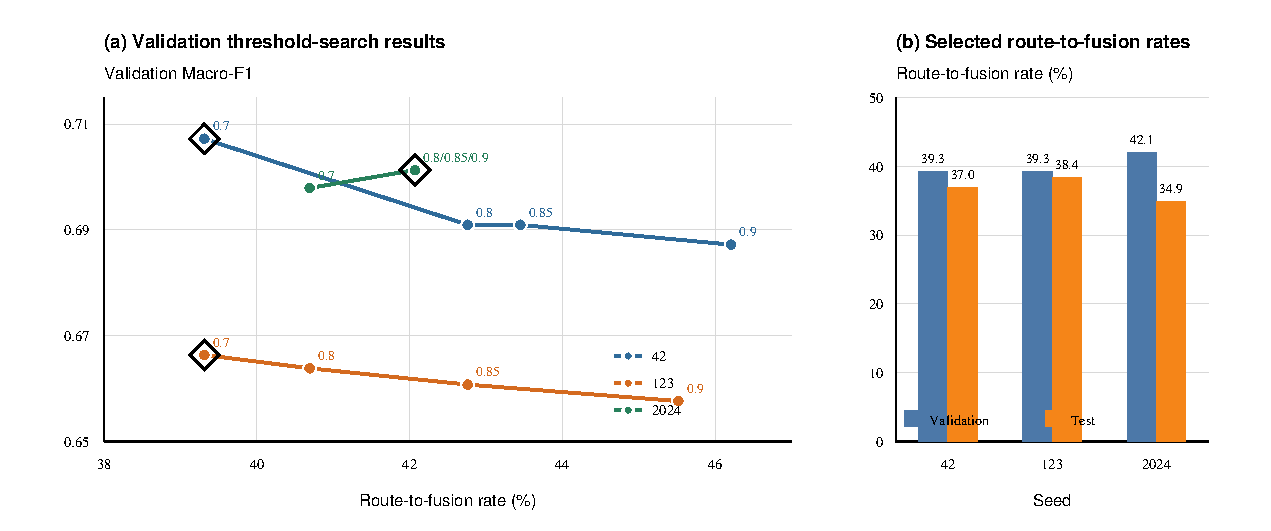
\includegraphics[width=\textwidth]{figures/serf_threshold_search_results.pdf}
\caption{Validation threshold-search results for SERF without augmentation. Panel (a) relates validation Macro-F1 to the route-to-fusion rate; labels denote \(\tau\), and outlined diamonds mark the validation-selected configurations. Panel (b) compares validation and test route-to-fusion rates at those configurations. All values are reproduced from the retained threshold-search table and seed-level test outputs.}
\label{fig:serf-threshold-search}
\end{figure}

Across the full \(\tau\) range, fusion coverage increased by 6.90 and 6.21 percentage points for seeds 42 and 123 while Macro-F1 decreased by 2.00 and 0.87 points; seed 2024 gained 0.34 Macro-F1 points for 1.38 points of additional fusion before plateauing. The pairs \((\tau,\delta)=(0.70,0.15)\), \((0.70,0.15)\), and \((0.80,0.15)\) were selected for seeds 42, 123, and 2024, respectively. Their validation fusion rates were 39.31\%, 39.31\%, and 42.07\%, compared with test rates of 36.99\%, 38.36\%, and 34.93\%. Test coverage was therefore lower for every seed, with the largest difference occurring at seed 2024. Moreover, \(\delta=0.15\) and \(0.20\) produced identical aggregate outcomes throughout the retained grid; selecting 0.15 consequently reflects a tie rather than evidence of a superior margin setting. Route-specific correctness was not retained, so this analysis characterizes threshold sensitivity and coverage rather than the separate accuracy of the easy and hard paths.

\begin{table}[!h]
\caption{Active-encoder complexity under different inference strategies.}\label{tab:active-encoder-complexity}
\centering
\setlength{\tabcolsep}{4pt}
\scriptsize
\resizebox{\textwidth}{!}{%
\begin{tabular}{lccc}
\toprule
\textbf{Inference strategy} & \textbf{Fusion rate} & \textbf{Active encoders per input} & \textbf{Reduction relative to static fusion} \\
\midrule
ELECTRA-only classifier & 0\% & 1.0000 & 50.00\% \\
SERF without augmentation & 36.76 \ensuremath{\pm} 1.72\% & 1.7352 \ensuremath{\pm} 0.0345 & 13.24 \ensuremath{\pm} 1.72\% \\
SERF with augmentation & 34.25 \ensuremath{\pm} 1.81\% & 1.6849 \ensuremath{\pm} 0.0362 & 15.75 \ensuremath{\pm} 1.81\% \\
Static ELECTRA--RoBERTa fusion & 100\% & 2.0000 & 0\% \\
\bottomrule
\end{tabular}
}
\end{table}

The lower fusion rate of the augmented configuration did not translate into better predictive performance; the unaugmented configuration therefore provided the more favorable observed balance. SERF bypassed fusion for approximately two-thirds of test requirements and required fewer active encoder invocations than static fusion, but more than an ELECTRA-only classifier. Its computational advantage is consequently conditional on comparison with always-on fusion.

\section{Performance Comparison and Discussion}\label{sec:performance-comparison}

Because augmentation conditions and repeated-run availability differed among configurations, all cross-model results are interpreted at the configuration level. The consequences for comparative validity are discussed in Sect.~\ref{sec:limitations}.

\subsection{Comparison with Single-Transformer Baselines}\label{sec:single-transformer-comparison}

The proposed SERF model was compared with four single-transformer baselines: BERT, ELECTRA, RoBERTa, and ModernBERT. The augmentation condition and number of retained runs are reported explicitly in Table~\ref{tab:single-transformer-comparison}.

\begin{table}[!h]
\caption{Comparison with single-transformer baselines.}\label{tab:single-transformer-comparison}
\centering
\setlength{\tabcolsep}{4pt}
\scriptsize
\resizebox{\textwidth}{!}{%
\begin{tabular}{lccccc}
\toprule
\textbf{Model} & \textbf{Augmentation} & \textbf{Runs} & \textbf{Accuracy} & \textbf{Weighted-F1} & \textbf{Macro-F1} \\
\midrule
BERT & Yes & 1 & 0.8500 & 0.8400 & 0.7100 \\
ELECTRA & No & 1 & 0.8425 & 0.8358 & 0.7205 \\
RoBERTa & No & 3 & 0.8379 \ensuremath{\pm} 0.0040 & 0.8348 \ensuremath{\pm} 0.0039 & 0.7279 \ensuremath{\pm} 0.0142 \\
ModernBERT & Yes & 1 & 0.8151 & 0.8103 & 0.7646 \\
\textbf{SERF} & No & 3 & \textbf{0.8653 \ensuremath{\pm} 0.0105} & \textbf{0.8595 \ensuremath{\pm} 0.0117} & \textbf{0.7770 \ensuremath{\pm} 0.0307} \\
\bottomrule
\end{tabular}
}
\end{table}

Only two-decimal classification results were retained for the BERT experiment. Values without standard deviations correspond to single-run results.

Overall, SERF achieved the highest recorded values across the reported metrics in the single-transformer comparison. The relative pattern across aggregate and macro-averaged measures suggests that selective fusion primarily benefited class-balanced classification rather than only majority-class performance.

\subsection{Comparison with Static Hybrid Models}\label{sec:static-hybrid-comparison}

SERF was further compared with two static hybrid configurations: the BERT--RoBERTa hybrid and the static ELECTRA--RoBERTa naive fusion model. Unlike SERF, these models activate both transformer encoders for every input. All three configurations were evaluated over the same three training seeds. The BERT--RoBERTa model used training-set augmentation, whereas the static ELECTRA--RoBERTa model and SERF were trained without augmentation.

\begin{table}[!h]
\caption{Comparison with static hybrid models.}\label{tab:static-hybrid-comparison}
\centering
\setlength{\tabcolsep}{4pt}
\scriptsize
\resizebox{\textwidth}{!}{%
\begin{tabular}{lccccccc}
\toprule
\textbf{Model} & \textbf{Augmentation} & \textbf{Runs} & \textbf{Accuracy} & \textbf{Weighted-F1} & \textbf{Macro Precision} & \textbf{Macro Recall} & \textbf{Macro-F1} \\
\midrule
BERT--RoBERTa & Yes & 3 & \textbf{0.8767 \ensuremath{\pm} 0.0181} & \textbf{0.8684 \ensuremath{\pm} 0.0198} & 0.7835 \ensuremath{\pm} 0.0421 & 0.7569 \ensuremath{\pm} 0.0348 & 0.7615 \ensuremath{\pm} 0.0409 \\
Static ELECTRA--RoBERTa & No & 3 & 0.8607 \ensuremath{\pm} 0.0172 & 0.8582 \ensuremath{\pm} 0.0227 & 0.8133 \ensuremath{\pm} 0.0319 & 0.7577 \ensuremath{\pm} 0.0725 & 0.7554 \ensuremath{\pm} 0.0577 \\
\textbf{SERF} & No & 3 & 0.8653 \ensuremath{\pm} 0.0105 & 0.8595 \ensuremath{\pm} 0.0117 & \textbf{0.8362 \ensuremath{\pm} 0.0340} & \textbf{0.7695 \ensuremath{\pm} 0.0366} & \textbf{0.7770 \ensuremath{\pm} 0.0307} \\
\bottomrule
\end{tabular}
}
\end{table}

Always-on fusion remained competitive on aggregate measures, whereas SERF achieved the strongest class-balanced result and avoided full fusion for most inputs. Section~\ref{sec:tradeoff} synthesizes this performance-efficiency trade-off.

\subsection{Macro-F1, Stability, and Complexity Trade-off}\label{sec:tradeoff}

No evaluated model family dominated classification performance, seed-level stability, and inference efficiency simultaneously. Single transformers required the fewest encoders, static hybrids remained competitive on aggregate measures, and SERF combined the strongest class-balanced result with intermediate active computation. Given the class imbalance, Macro-F1 remains the principal comparison criterion, while SERF's efficiency advantage applies to always-on fusion rather than single-transformer inference.

\subsection{Error Analysis on Minority Classes}\label{sec:minority-error-analysis}

Several minority classes contained only two to five test instances. Consequently, a single correct or incorrect prediction could substantially change the corresponding per-class F1 score and the overall Macro-F1. The reported ranges should therefore be interpreted as support-sensitive descriptive results rather than robust estimates of minority-class generalization.

\begin{table}[!h]
\caption{Class-level F1 ranges across the three SERF seeds.}\label{tab:class-f1-ranges}
\centering
\setlength{\tabcolsep}{4pt}
\scriptsize
\begin{tabularx}{\textwidth}{lCCC}
\toprule
\textbf{Class} & \textbf{Test support} & \textbf{Without augmentation} & \textbf{With augmentation} \\
\midrule
F (majority reference) & 67 & 0.91--0.95 & 0.89--0.91 \\
A & 5 & 0.57--0.75 & 0.57--0.75 \\
FT & 2 & 0.67--1.00 & 0.57--0.80 \\
L & 2 & 0.80--1.00 & 1.00 \\
MN & 3 & 0.40--0.75 & 0.33--0.67 \\
PO & 2 & 0.50--0.67 & 0.00--0.67 \\
SC & 3 & 0.80 & 0.50 \\
\bottomrule
\end{tabularx}
\end{table}

\clearpage
\begin{figure}[!t]
\centering
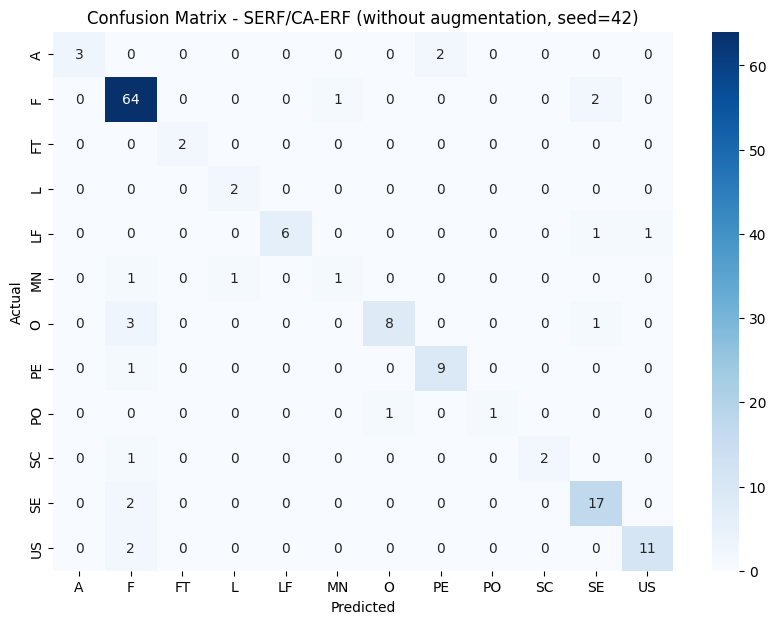
\includegraphics[width=0.49\textwidth]{figures/confusionseed42.png}\hfill
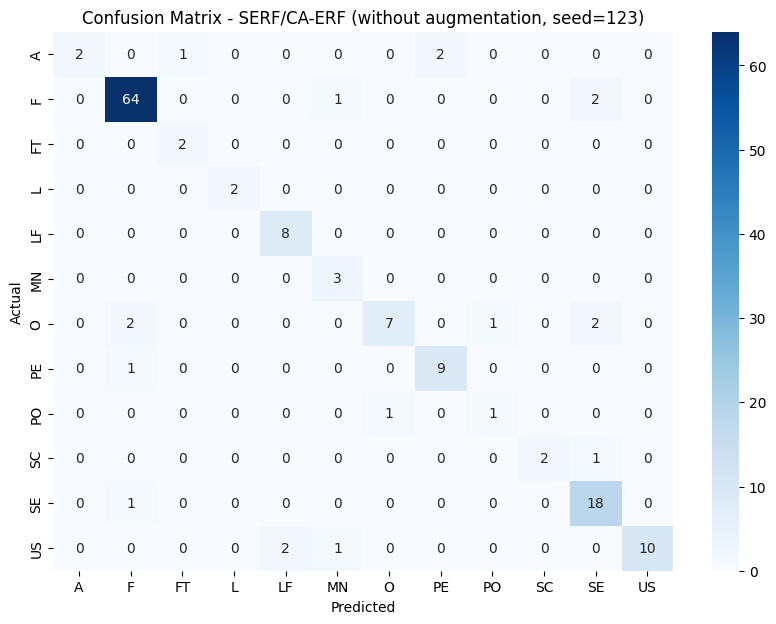
\includegraphics[width=0.49\textwidth]{figures/seed123.png}

\vspace{0.5em}
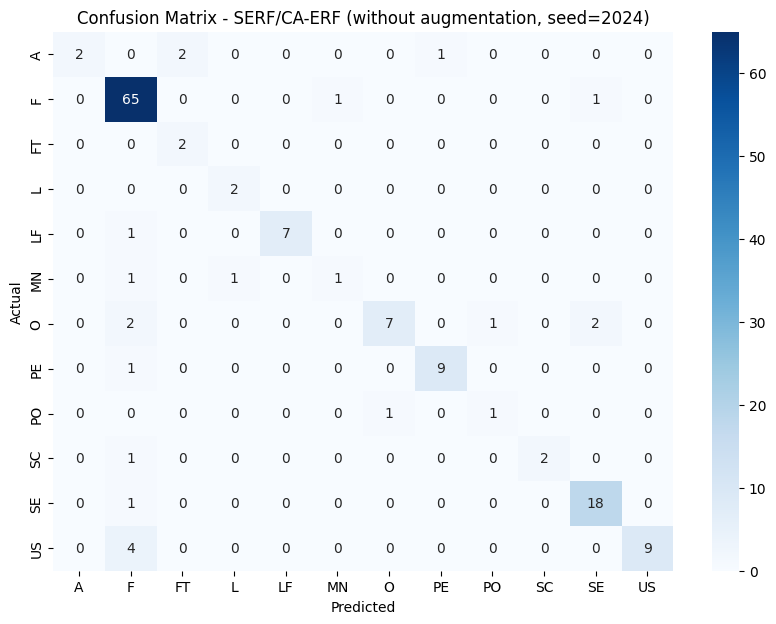
\includegraphics[width=0.49\textwidth]{figures/confusionseed2024.png}
\caption{Test-set confusion matrices retained for SERF/CA-ERF without augmentation at seeds 42, 123, and 2024. Rows denote actual classes, columns denote predicted classes, and cell annotations are prediction counts for the same 146-instance test partition.}
\label{fig:serf-confusion-seeds}
\end{figure}

The seed-level matrices in Fig.~\ref{fig:serf-confusion-seeds} show that A was correctly identified in three, two, and two of its five test cases at seeds 42, 123, and 2024, respectively; the remaining cases were assigned to PE or FT. SC retained two correct predictions in every run, with its remaining case assigned to F at seeds 42 and 2024 and to SE at seed 123. PO exhibited the same pattern in all three runs: one correct prediction and one assignment to O. F was comparatively stable, with 64, 64, and 65 correct predictions out of 67. Recurring O errors involved F and SE, whereas US errors varied across seeds, occurring mainly as F at seeds 42 and 2024 and as LF or MN at seed 123. These variations are consistent with the sensitivity of low-support classes to individual predictions.

The retained confusion matrices support class-level error counts but do not contain the instance-level predictions, route decisions, or normalized requirement texts needed for deeper analysis. Consequently, they cannot determine the linguistic characteristics associated with these confusion pairs or whether specific errors originated on the easy or hard path. These questions require prediction-level outputs in future experiments.

\section{Discussion}\label{sec:discussion}

\subsection{Key Findings}\label{sec:key-findings}

The non-uniform augmentation response indicates that synthetic balancing interacts with the model configuration rather than providing a consistent benefit. A plausible explanation is that lexical transformations can alter modal expressions, numerical constraints, or domain-specific cues that carry substantial meaning in short requirements. The failure of validation gains to transfer to the test set further suggests sensitivity to the selected synthetic distribution, although the retained outputs do not establish the causal mechanism.

The concentration of errors in low-support classes is consistent with insufficient evidence for learning stable minority-class boundaries. The difference between macro precision and macro recall further indicates conservative minority-class decisions, with false negatives remaining more persistent than false positives. Consequently, further improvements should prioritize minority-class recall rather than majority-class accuracy.

The threshold grid shows that greater fusion coverage did not consistently improve validation Macro-F1. The two tested margin settings were indistinguishable at the aggregate level, while selected validation coverage did not transfer exactly to the test partition. Routing therefore remains sensitive to the confidence threshold, model initialization, and evaluation partition; the current experiments do not isolate the individual contributions of confidence, margin, and the risky-class check. The limited number of repeated runs also precludes a strong statistical conclusion about comparative stability.

\subsection{Practical Implications}\label{sec:practical-implications}

SERF may support batch triage or resource-constrained classification when always-on dual-encoder inference is unnecessary. Fusion-routed requirements can be prioritized for analyst review, making SERF a decision-support component rather than a replacement for analysts, particularly for low-support or high-impact classes. Deployment benefits require matched latency, throughput, memory, and energy measurements; moreover, uncalibrated confidence and margin values should be treated as routing signals rather than correctness probabilities.

Routing thresholds should be selected on validation data representative of the deployment domain because the selected values varied across seeds. Macro Recall, per-class F1, route-to-fusion rate, and minority-class predictions should be monitored jointly. Synthetic balancing should likewise be retained only when configuration-specific validation gains transfer to unchanged evaluation data.

\subsection{Limitations}\label{sec:limitations}

The first limitation concerns the small and highly imbalanced benchmark. Several classes have minimal test support, making per-class metrics highly sensitive to individual predictions and preventing strong conclusions about minority-class generalization.

The experiments used a stratified random split rather than a project-disjoint evaluation. Requirements originating from related projects may share vocabulary and writing conventions. Therefore, the reported results do not establish generalization to entirely unseen software projects. A project-wise or leave-one-project-out protocol would provide a stronger assessment of cross-project transfer.

The evaluation protocol was not fully uniform across all baseline models. The primary models were evaluated through repeated runs, whereas several baseline and augmentation experiments retained only single-run outputs. Model configurations and augmentation conditions also differed, and some baseline results were stored only as rounded classification reports. In addition, route-specific correctness and component-wise routing ablations were not retained, preventing isolation of the confidence, margin, and risky-class mechanisms. Consequently, the comparisons support descriptive conclusions but not statistical significance or architecture-only causality.

The computational analysis used active encoder invocations as a proxy. This measure does not account for differences in encoder size, sequence-processing cost, GPU utilization, memory consumption, energy use, or batching behavior. In addition, identically instrumented latency measurements were not retained for every baseline. The estimated computational reduction should therefore not be interpreted as an equivalent reduction in wall-clock latency or FLOPs.

The augmentation analysis is also limited by minor implementation differences across the baseline notebooks and by the absence of manual semantic-quality assessment for generated requirements. Although augmentation was restricted to the training set, the experiments did not verify whether every synthetic requirement preserved the intent and class semantics of its source.

\section{Conclusion and Future Work}\label{sec:conclusion}

\subsection*{Summary of contributions}\label{sec:summary-contributions}

This study developed and evaluated SERF, which retains ELECTRA predictions for easy cases and invokes an independent ELECTRA--RoBERTa fusion branch for uncertain or predefined risky-class cases. Comparisons with single-encoder and static-hybrid configurations examined class-balanced performance, seed-level stability, augmentation response, and active encoder demand.

\subsection*{Answers to research questions}\label{sec:answers-rqs}

\emph{\textbf{RQ1: How effectively can pretrained transformer models classify software requirements across functional and multiple non-functional categories under class imbalance?}}

Pretrained transformers provided useful multiclass performance on PROMISE\_EXP, but the gap between weighted and macro-averaged measures shows that reliability remained uneven across classes. Overall accuracy is therefore insufficient for evaluating this imbalanced task.

\emph{\textbf{RQ2: How does the proposed SERF model compare with single-encoder and static hybrid transformer baselines in terms of class-balanced performance and seed-level stability?}}

SERF recorded the highest mean Macro-F1 among the primary three-seed comparisons, whereas RoBERTa showed the lowest Macro-F1 variation and static fusion remained competitive on aggregate metrics. The observed SERF advantage was therefore concentrated in class-balanced performance and should not be interpreted as statistical or universal superiority.

\emph{\textbf{RQ3: How do confidence- and class-aware selective routing and training-set augmentation affect classification performance and active inference demand?}}

SERF routed \(36.76\% \pm 1.72\%\) of test requirements to fusion, yielding an estimated 13.24\% reduction in active encoder invocations relative to static fusion, but not relative to a single encoder. More routing did not consistently improve validation Macro-F1, and the two tested margin settings produced identical aggregate outcomes. The individual routing components therefore remain unisolated, while augmentation reduced test Macro-F1; both routing and augmentation should be validated against predictive performance rather than fusion rate or confidence alone.

\subsection*{Future research directions}\label{sec:future-work}

Future research should evaluate SERF on additional datasets and project-disjoint splits using repeated cross-validation, additional seeds, and paired statistical tests. Efficiency should be assessed through matched latency, throughput, FLOPs, peak-memory, and energy measurements; reusing the selector's ELECTRA representation, calibrating confidence, broadening the threshold search, and conducting component-wise routing ablations may further improve routing.

The effect of augmentation should be examined through class-specific ablations and semantic-quality assessment of generated samples. Prediction-level outputs and route decisions should also be retained for confusion and routing-error analysis. Finally, token-level attribution, controlled feature masking, and qualitative error inspection are needed to address the still-open question of which lexical and contextual features influence the encoders.

\appendix

\section{Software and Hardware Environment}\label{app:software-reproducibility}

The experimental implementation used the following software libraries:

\begin{itemize}
\item \textbf{PyTorch} \cite{paszke_pytorch}: neural network construction, data loading, class-weighted loss computation, automatic mixed precision, gradient accumulation, and optimization.
\item \textbf{Hugging Face Transformers} \cite{wolf_transformers}: pretrained tokenizers and encoders, including BERT, RoBERTa, ELECTRA, and ModernBERT. The Trainer and TrainingArguments interfaces were used for several baseline and hybrid models.
\item \textbf{Scikit-learn} \cite{pedregosa_scikit}: stratified dataset splitting, label encoding, balanced class-weight calculation, classification metrics, classification reports, and confusion matrices.
\item \textbf{Pandas and NumPy:} dataset manipulation, result aggregation, and calculation of the mean and standard deviation across experimental seeds.
\item \textbf{NLTK:} WordNet-based synonym replacement and training-set augmentation.
\item \textbf{Matplotlib and Seaborn:} visualization of training histories and confusion matrices.
\end{itemize}

The experimental notebooks do not consistently pin exact package versions. The SERF and selected ELECTRA--RoBERTa notebooks constrain Transformers to versions greater than or equal to 4.48 and below 5, whereas other notebooks use open-ended lower bounds or package-update commands without complete version constraints. Consequently, the exact software environment is not explicitly specified in the retained experiments and should be documented through an environment snapshot in future replication studies.

The notebooks were executed in Google Colab and selected a CUDA device when available, with a CPU fallback. FP16, BF16, or CUDA automatic mixed precision was enabled according to the model implementation and hardware support.

The exact GPU model, GPU memory, CPU specification, system RAM, Colab runtime tier, and driver configuration are not explicitly specified in the current experiments. Consequently, a specific accelerator such as a Tesla T4, L4, V100, or A100 should not be reported without checking the original Colab runtime logs.

\section{Detailed Model and Training Configurations}\label{app:training-configurations}

The custom ELECTRA, static ELECTRA-RoBERTa, and SERF implementations used AdamW. For models trained through Hugging Face Trainer, the optimizer was determined by the corresponding Trainer configuration and installed Transformers version. A linear learning-rate schedule with a 10\% warm-up period was explicitly implemented for standalone ELECTRA.

Gradient clipping with a maximum norm of 1.0 was explicitly applied to ELECTRA and the hybrid models. Gradient checkpointing was enabled for static ELECTRA-RoBERTa and SERF.

Balanced class weights were computed from the training frame used by each experimental variant:

\[ w_k=\frac{N_{\mathrm{tr}}}{K n_k}, \]

where \(N_{\mathrm{tr}}\) is the number of training instances, \(K\) is the number of classes, and \(n_k\) is the number of training instances belonging to class \(k\).

The explicitly defined classifier-head dropout rates were 0.1 for BERT and RoBERTa, 0.5 for BERT-RoBERTa, 0.3 for ModernBERT-ELECTRA, and 0.2 for ELECTRA-RoBERTa and SERF. In the frozen variants, encoder layers 0-7 were frozen, while the higher Transformer layers and classifier head remained trainable \cite{said_functional_nonfunctional}.

\subsection*{Preprocessing and augmentation details}

Minimal normalization removed duplicated whitespace and standardized textual format where necessary. Stemming, stop-word removal, punctuation removal, and digit removal were not applied because modal verbs, numerical constraints, and domain-specific tokens may distinguish requirement classes.

The augmentation procedure comprised synonym replacement, phrase insertion, text simplification, random word swapping, and random word deletion. These transformations were applied only to the training partition. Transformer class weights were incorporated into cross-entropy loss and computed from the training distribution of the corresponding variant.

For augmented experiments, the training support of FT, L, MN, A, LF, SC, PO, PE, O, and US was increased to 200 instances, while SE was increased to 100 instances.

\subsection*{Static-fusion and routing details}

The static ELECTRA--RoBERTa model independently encoded each requirement and extracted the 768-dimensional first-token representation from each encoder. The representations were concatenated before dropout, layer normalization, a linear projection from 1536 to 768 dimensions, GELU activation, additional dropout, and final classification \cite{said_functional_nonfunctional}.

The SERF selector and fusion branch were trained separately. Validation-only threshold selection evaluated

\[ \tau\in\{0.70,0.80,0.85,0.90\},\qquad \delta\in\{0.15,0.20\}. \]

The pair maximizing validation Macro-F1 was selected, with route-to-fusion rate and accuracy serving as secondary tie-breaking criteria. The risky-class set was \(\{\mathrm{A,L,FT,MN,PO,SC,PE,O,US}\}\).

\begin{table}[!hb]
\caption{Model configurations.}\label{tab:model-configurations}
\centering
\setlength{\tabcolsep}{4pt}
\scriptsize
\resizebox{\textwidth}{!}{%
\begin{tabular}{lcccccccc}
\toprule
\textbf{Model} & \textbf{Learning rate} & \textbf{Epochs} & \textbf{Train/ Eval batch} & \textbf{Gradient accumulation} & \textbf{Effective train batch} & \textbf{Weight decay} & \textbf{Precision} & \textbf{Frozen layers} \\
\midrule
BERT / RoBERTa & \(1\times10^{-5}\) & 30 & 16 / 16 & 2 & 32 & 0.10 / 0.02 & FP16 & Lower 8 layers \\
ELECTRA & \(2\times10^{-5}\) & 30 & 16 / 32 & 1 & 16 & 0.10 / 0.01 & Not explicitly specified & Lower 8 layers \\
ModernBERT & \(2\times10^{-5}\) & 30 & 16 / 16 & 2 & 32 & 0.10 / 0.01 & BF16 if supported; otherwise FP16 & Lower 8 layers \\
ModernBERT, no-freeze variant & \(2\times10^{-5}\) & 30 & 16 / 16 & 2 & 32 & 0.10 / 0.01 & BF16 if supported; otherwise FP16 & None \\
BERT--RoBERTa & \(1\times10^{-5}\) & 30 & 16 / 16 & 2 & 32 & 0.10 / 0.02 & FP16 when CUDA is available & Lower 8 layers per encoder \\
ModernBERT--ELECTRA & \(1\times10^{-5}\) or \(2\times10^{-5}\) & 30 & 1 / 1 & 8 & 8 & 0.10 / 0.02 & FP16 when CUDA is available & Lower 8 layers per encoder \\
Static ELECTRA--RoBERTa & \(2\times10^{-5}\) & Up to 30 & 4 / 16 & 4 & 16 & Not used / 0.01 & CUDA AMP & Lower 8 layers per encoder \\
SERF selector and fusion branch & \(2\times10^{-5}\) & 30 per stage & 4 / 16 & 4 & 16 & Not used / 0.01 & CUDA AMP & Lower 8 layers per encoder \\
\bottomrule
\end{tabular}
}
\end{table}

\section{Evaluation Definitions and Complexity Derivation}\label{app:evaluation-definitions}

For class \(k\), precision, recall, and F1 are defined as:

\[ P_k=\frac{TP_k}{TP_k+FP_k},\qquad R_k=\frac{TP_k}{TP_k+FN_k}, \]\[ F1_k=\frac{2P_kR_k}{P_k+R_k}. \]

Undefined values were assigned zero, consistent with zero\_division=0 in the experimental implementation. Overall accuracy is:

\[ \mathrm{Accuracy} =\frac{1}{N}\sum_{i=1}^{N}\mathbb{I}(y_i=\hat{y}_i). \]

Macro-averaged metrics are:

\[ P_{\mathrm{macro}}=\frac{1}{K}\sum_{k=1}^{K}P_k,\qquad R_{\mathrm{macro}}=\frac{1}{K}\sum_{k=1}^{K}R_k, \]\[ F1_{\mathrm{macro}}=\frac{1}{K}\sum_{k=1}^{K}F1_k. \]

Weighted F1 is:

\[ F1_{\mathrm{weighted}} =\sum_{k=1}^{K}\frac{n_k}{N}F1_k. \]

For SERF, the route-to-fusion indicator is:

\[ z_i=\mathbb{I}\left( c_i<\tau\;\lor\; m_i<\delta\;\lor\; \hat{y}^{E}_i\in\mathcal{R} \right), \]

where \(c_i\) is the maximum ELECTRA softmax probability, \(m_i\) is the difference between the two highest probabilities, and \(\mathcal{R}\) is the risky-class set. The route-to-fusion rate is:

\[ r=\frac{1}{N}\sum_{i=1}^{N}z_i. \]

For three-seed experiments:

\[ \bar{x}=\frac{1}{S}\sum_{s=1}^{S}x_s,\qquad s_x=\sqrt{\frac{1}{S-1}\sum_{s=1}^{S}(x_s-\bar{x})^2}, \]

where \(S=3\). Since no significance test or confidence interval was implemented, the mean and standard deviation are interpreted descriptively.

\subsection*{Active-encoder complexity derivation}

In the implemented architecture, an easy-path prediction requires one ELECTRA encoder invocation, while a hard-path prediction requires three invocations: the ELECTRA selector, the ELECTRA encoder in the fusion model, and the RoBERTa encoder. Thus,

\[C_{\mathrm{SERF}}=(1-r)C_{\mathrm{easy}}+rC_{\mathrm{hard}}=(1-r)+3r=1+2r.\]

The always-on static ELECTRA--RoBERTa fusion model activates two encoders for every requirement, giving \(C_{\mathrm{static}}=2\). The relative reduction in active encoder invocations is

\[R_{\mathrm{encoder}}=\frac{C_{\mathrm{static}}-C_{\mathrm{SERF}}}{C_{\mathrm{static}}}\times100\%.\]

Using the mean route-to-fusion rate of 0.3676, SERF required 1.7352 active encoder invocations per requirement and produced the following estimate relative to static fusion:

\[R_{\mathrm{encoder}}=\frac{2-1.7352}{2}\times100\%=13.24\%.\]

The selective architecture is less expensive than static fusion when \(r<0.5\), because \(1+2r<2\); all three evaluated seeds satisfied this condition. This proxy does not measure FLOPs, latency, energy consumption, or memory usage, and it excludes tokenization because both tokenized views were prepared before routing.

\subsection*{Descriptive inference timing}

The routed test stage of the unaugmented SERF configuration required \(1.9448\pm0.0369\) seconds for 146 test instances in the recorded experimental environment, corresponding to approximately 13.32 ms per instance. Identically instrumented timings were not retained for all baselines; therefore, this result is descriptive and does not support a claim of comparative latency superiority.

\clearpage
\section{SERF Routing Architecture}\label{app:serf-routing-architecture}

\begin{figure}[!ht]
\centering
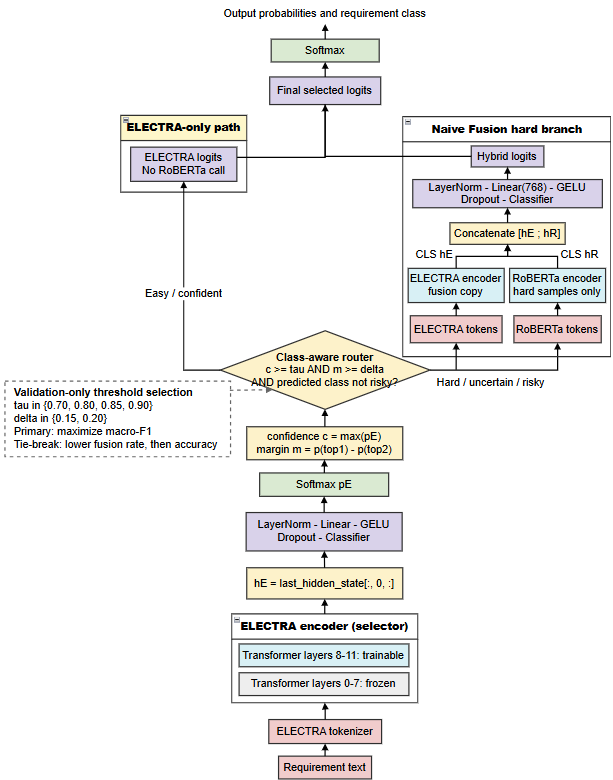
\includegraphics[width=0.72\textwidth]{figures/serf_routing_architecture.png}
\caption{Detailed architecture of the SERF confidence router and selective fusion paths. Both tokenized views are prepared before routing in the implemented data pipeline; only encoder invocation is selective.}
\label{fig:serf-routing-architecture}
\end{figure}

\clearpage
\section{Supplementary Augmentation Results}\label{app:supplementary-augmentation}

\begin{table}[!h]
\caption{Descriptive comparison of augmentation effects across model configurations at seed 42.}\label{tab:augmentation-models-seed42}
\centering
\setlength{\tabcolsep}{4pt}
\scriptsize
\begin{tabularx}{\textwidth}{Yccc}
\toprule
\textbf{Model configuration} & \textbf{Without augmentation} & \textbf{With augmentation} & \textbf{Difference} \\
\midrule
BERT & 0.5900 & 0.7100 & +0.1200 \\
ELECTRA & 0.7205 & 0.6337 & \ensuremath{-}0.0869 \\
RoBERTa & 0.7176 & 0.6800 & \ensuremath{-}0.0376 \\
ModernBERT & 0.7050 & 0.7646 & +0.0596 \\
Hybrid BERT--RoBERTa & 0.5900 & 0.7146 & +0.1246 \\
Static ELECTRA--RoBERTa fusion & 0.7953 & 0.7286 & \ensuremath{-}0.0667 \\
SERF & 0.7942 & 0.6611 & \ensuremath{-}0.1331 \\
\bottomrule
\end{tabularx}
\end{table}

BERT results, RoBERTa with augmentation, and BERT--RoBERTa without augmentation were retained only to two decimal places. Differences involving these results inherit the same precision limitation.

Across models, augmentation had no consistent directional effect. Complete paired multi-seed results were unavailable for every baseline; therefore, the comparison is descriptive and does not establish architecture-dependent causality.

% ---- Bibliography ----
% Preserve source bibliography entries R8 and R9, which are not cited in the paper body.
\nocite{tahir_cross_project_requirements,hemmat_llm_requirements}
\bibliographystyle{splncs04}
\bibliography{references}

\end{document}
